\documentclass{book}
\usepackage[a4paper,top=2.5cm,bottom=2.5cm,left=2.5cm,right=2.5cm]{geometry}
\usepackage{makeidx}
\usepackage{natbib}
\usepackage{graphicx}
\usepackage{multicol}
\usepackage{float}
\usepackage{listings}
\usepackage{color}
\usepackage{ifthen}
\usepackage[table]{xcolor}
\usepackage{textcomp}
\usepackage{alltt}
\usepackage{ifpdf}
\ifpdf
\usepackage[pdftex,
            pagebackref=true,
            colorlinks=true,
            linkcolor=blue,
            unicode
           ]{hyperref}
\else
\usepackage[ps2pdf,
            pagebackref=true,
            colorlinks=true,
            linkcolor=blue,
            unicode
           ]{hyperref}
\usepackage{pspicture}
\fi
\usepackage[utf8]{inputenc}
\usepackage[spanish]{babel}
\usepackage{mathptmx}
\usepackage[scaled=.90]{helvet}
\usepackage{courier}
\usepackage{sectsty}
\usepackage{amssymb}
\usepackage[titles]{tocloft}
\usepackage{doxygen}
\lstset{language=C++,inputencoding=utf8,basicstyle=\footnotesize,breaklines=true,breakatwhitespace=true,tabsize=2,numbers=left }
\makeindex
\setcounter{tocdepth}{3}
\renewcommand{\footrulewidth}{0.4pt}
\renewcommand{\familydefault}{\sfdefault}
\hfuzz=15pt
\setlength{\emergencystretch}{15pt}
\hbadness=750
\tolerance=750
\begin{document}
\hypersetup{pageanchor=false,citecolor=blue}
\begin{titlepage}
\vspace*{7cm}
\begin{center}
{\Large Laboratorio de P\-R\-O2. Ejercicio Factor P\-S\-I \\[1ex]\large version oct-\/2013 }\\
\vspace*{1cm}
{\large Generado por Doxygen 1.8.2}\\
\vspace*{0.5cm}
{\small Lunes, 17 de Marzo de 2014 17:34:40}\\
\end{center}
\end{titlepage}
\clearemptydoublepage
\pagenumbering{roman}
\tableofcontents
\clearemptydoublepage
\pagenumbering{arabic}
\hypersetup{pageanchor=true,citecolor=blue}
\chapter{Ejemplo de diseño modular\-: Factor Psi.}
\label{index}\hypertarget{index}{}En este ejemplo se construye un programa modular que ofrece un menú de opciones para gestionar una lavadora. Se introducen las clases {\itshape \hyperlink{class_lavadora}{Lavadora}}, {\itshape \hyperlink{class_cubeta}{Cubeta}} y {\itshape \hyperlink{class_prenda}{Prenda}}. 
\chapter{Índice de clases}
\section{Lista de clases}
Lista de las clases, estructuras, uniones e interfaces con una breve descripción\-:\begin{DoxyCompactList}
\item\contentsline{section}{\hyperlink{class_cjt__organismes}{Cjt\-\_\-organismes} \\*Conté un conjunt d'organismes }{\pageref{class_cjt__organismes}}{}
\item\contentsline{section}{\hyperlink{class_organisme}{Organisme} \\*Contiene celulas ordenadas }{\pageref{class_organisme}}{}
\end{DoxyCompactList}

\chapter{Indice de archivos}
\section{Lista de archivos}
Lista de todos los archivos con descripciones breves\-:\begin{DoxyCompactList}
\item\contentsline{section}{\hyperlink{_lista_palabras_8hpp}{Lista\-Palabras.\-hpp} \\*Especificación de la clase \hyperlink{class_lista_palabras}{Lista\-Palabras} }{\pageref{_lista_palabras_8hpp}}{}
\item\contentsline{section}{\hyperlink{_palabra_8hpp}{Palabra.\-hpp} \\*Especificación de la clase \hyperlink{class_palabra}{Palabra} }{\pageref{_palabra_8hpp}}{}
\item\contentsline{section}{\hyperlink{pro2__s52_8cpp}{pro2\-\_\-s52.\-cpp} \\*Programa principal para el ejercicio {\itshape Factor Psi} }{\pageref{pro2__s52_8cpp}}{}
\end{DoxyCompactList}

\chapter{Documentación de las clases}
\hypertarget{class_lista_palabras}{\section{Referencia de la Clase Lista\-Palabras}
\label{class_lista_palabras}\index{Lista\-Palabras@{Lista\-Palabras}}
}


Representa una colección de palabras distintas, cada una con un natural asociado.  


\subsection*{Métodos públicos}
\begin{DoxyCompactItemize}
\item 
\hyperlink{class_lista_palabras_ae0d9e5a9aa149270056f47d272f36460}{Lista\-Palabras} ()
\begin{DoxyCompactList}\small\item\em Creadora por defecto. \end{DoxyCompactList}\item 
void \hyperlink{class_lista_palabras_a1321849c60c36bd29208103984a37192}{anadir\-\_\-palabra} (const \hyperlink{class_palabra}{Palabra} \&p)
\begin{DoxyCompactList}\small\item\em Añade una palabra a la lista. \end{DoxyCompactList}\item 
int \hyperlink{class_lista_palabras_ad593a5988b7ec974e9621e8cd26e0e06}{longitud} () const 
\begin{DoxyCompactList}\small\item\em Consultora de la longitud. \end{DoxyCompactList}\item 
int \hyperlink{class_lista_palabras_aaafa09ef438a8ee956d2c1a095e578f4}{max\-\_\-frec} () const 
\begin{DoxyCompactList}\small\item\em Consultora de la frecuencia de la palabra más frecuente. \end{DoxyCompactList}\item 
void \hyperlink{class_lista_palabras_ac4d573f9174b86d307dfb06af8db5e1f}{escribir\-\_\-lista} () const 
\begin{DoxyCompactList}\small\item\em Operación de escritura. \end{DoxyCompactList}\end{DoxyCompactItemize}
\subsection*{Métodos públicos estáticos}
\begin{DoxyCompactItemize}
\item 
static int \hyperlink{class_lista_palabras_a0ecc807102c0e8319da3f1c229e1325c}{longitud\-\_\-maxima} ()
\begin{DoxyCompactList}\small\item\em Consultora de la longitud máxima. \end{DoxyCompactList}\end{DoxyCompactItemize}


\subsection{Descripción detallada}
Representa una colección de palabras distintas, cada una con un natural asociado. 

El natural representa el número de veces que la palabra se ha añadido a la lista, lo consideramos la {\itshape frecuencia} de dicha palabra 

Definición en la línea 21 del archivo Lista\-Palabras.\-hpp.



\subsection{Documentación del constructor y destructor}
\hypertarget{class_lista_palabras_ae0d9e5a9aa149270056f47d272f36460}{\index{Lista\-Palabras@{Lista\-Palabras}!Lista\-Palabras@{Lista\-Palabras}}
\index{Lista\-Palabras@{Lista\-Palabras}!ListaPalabras@{Lista\-Palabras}}
\subsubsection[{Lista\-Palabras}]{\setlength{\rightskip}{0pt plus 5cm}Lista\-Palabras\-::\-Lista\-Palabras (
\begin{DoxyParamCaption}
{}
\end{DoxyParamCaption}
)}}\label{class_lista_palabras_ae0d9e5a9aa149270056f47d272f36460}


Creadora por defecto. 

Se ejecuta automáticamente al declarar una lista.

\begin{DoxyPrecond}{Precondición}
cierto 
\end{DoxyPrecond}
\begin{DoxyPostcond}{Postcondición}
El resultado es una lista vacía 
\end{DoxyPostcond}


\subsection{Documentación de las funciones miembro}
\hypertarget{class_lista_palabras_a1321849c60c36bd29208103984a37192}{\index{Lista\-Palabras@{Lista\-Palabras}!anadir\-\_\-palabra@{anadir\-\_\-palabra}}
\index{anadir\-\_\-palabra@{anadir\-\_\-palabra}!ListaPalabras@{Lista\-Palabras}}
\subsubsection[{anadir\-\_\-palabra}]{\setlength{\rightskip}{0pt plus 5cm}void Lista\-Palabras\-::anadir\-\_\-palabra (
\begin{DoxyParamCaption}
\item[{const {\bf Palabra} \&}]{p}
\end{DoxyParamCaption}
)}}\label{class_lista_palabras_a1321849c60c36bd29208103984a37192}


Añade una palabra a la lista. 

\begin{DoxyPrecond}{Precondición}
La longitud del parámetro implícito es menor que la longitud máxima o {\itshape p} ya está en él 
\end{DoxyPrecond}
\begin{DoxyPostcond}{Postcondición}
Si {\itshape p} está en el parámetro implícito, su frecuencia queda incrementada en una unidad, si no, aparece en él con frecuencia 1 
\end{DoxyPostcond}
\hypertarget{class_lista_palabras_a0ecc807102c0e8319da3f1c229e1325c}{\index{Lista\-Palabras@{Lista\-Palabras}!longitud\-\_\-maxima@{longitud\-\_\-maxima}}
\index{longitud\-\_\-maxima@{longitud\-\_\-maxima}!ListaPalabras@{Lista\-Palabras}}
\subsubsection[{longitud\-\_\-maxima}]{\setlength{\rightskip}{0pt plus 5cm}static int Lista\-Palabras\-::longitud\-\_\-maxima (
\begin{DoxyParamCaption}
{}
\end{DoxyParamCaption}
)\hspace{0.3cm}{\ttfamily [static]}}}\label{class_lista_palabras_a0ecc807102c0e8319da3f1c229e1325c}


Consultora de la longitud máxima. 

\begin{DoxyPrecond}{Precondición}
cierto 
\end{DoxyPrecond}
\begin{DoxyPostcond}{Postcondición}
El resultado es la longitud máxima de una lista permitida por la implementación 
\end{DoxyPostcond}
\hypertarget{class_lista_palabras_ad593a5988b7ec974e9621e8cd26e0e06}{\index{Lista\-Palabras@{Lista\-Palabras}!longitud@{longitud}}
\index{longitud@{longitud}!ListaPalabras@{Lista\-Palabras}}
\subsubsection[{longitud}]{\setlength{\rightskip}{0pt plus 5cm}int Lista\-Palabras\-::longitud (
\begin{DoxyParamCaption}
{}
\end{DoxyParamCaption}
) const}}\label{class_lista_palabras_ad593a5988b7ec974e9621e8cd26e0e06}


Consultora de la longitud. 

\begin{DoxyPrecond}{Precondición}
cierto 
\end{DoxyPrecond}
\begin{DoxyPostcond}{Postcondición}
El resultado es la longitud del parámetro implícito 
\end{DoxyPostcond}
\hypertarget{class_lista_palabras_aaafa09ef438a8ee956d2c1a095e578f4}{\index{Lista\-Palabras@{Lista\-Palabras}!max\-\_\-frec@{max\-\_\-frec}}
\index{max\-\_\-frec@{max\-\_\-frec}!ListaPalabras@{Lista\-Palabras}}
\subsubsection[{max\-\_\-frec}]{\setlength{\rightskip}{0pt plus 5cm}int Lista\-Palabras\-::max\-\_\-frec (
\begin{DoxyParamCaption}
{}
\end{DoxyParamCaption}
) const}}\label{class_lista_palabras_aaafa09ef438a8ee956d2c1a095e578f4}


Consultora de la frecuencia de la palabra más frecuente. 

\begin{DoxyPrecond}{Precondición}
cierto 
\end{DoxyPrecond}
\begin{DoxyPostcond}{Postcondición}
El resultado es la frecuencia de la palabra más frecuente del parámetro implícito 
\end{DoxyPostcond}
\hypertarget{class_lista_palabras_ac4d573f9174b86d307dfb06af8db5e1f}{\index{Lista\-Palabras@{Lista\-Palabras}!escribir\-\_\-lista@{escribir\-\_\-lista}}
\index{escribir\-\_\-lista@{escribir\-\_\-lista}!ListaPalabras@{Lista\-Palabras}}
\subsubsection[{escribir\-\_\-lista}]{\setlength{\rightskip}{0pt plus 5cm}void Lista\-Palabras\-::escribir\-\_\-lista (
\begin{DoxyParamCaption}
{}
\end{DoxyParamCaption}
) const}}\label{class_lista_palabras_ac4d573f9174b86d307dfb06af8db5e1f}


Operación de escritura. 

\begin{DoxyPrecond}{Precondición}
cierto 
\end{DoxyPrecond}
\begin{DoxyPostcond}{Postcondición}
El parámetro implícito se ha escrito en el canal estandar de salida 
\end{DoxyPostcond}


La documentación para esta clase fue generada a partir del siguiente fichero\-:\begin{DoxyCompactItemize}
\item 
\hyperlink{_lista_palabras_8hpp}{Lista\-Palabras.\-hpp}\end{DoxyCompactItemize}

\hypertarget{class_palabra}{\section{Referencia de la Clase Palabra}
\label{class_palabra}\index{Palabra@{Palabra}}
}


Representa una lista indexada de caracteres alfanuméricos.  


\subsection*{Métodos públicos}
\begin{DoxyCompactItemize}
\item 
\hyperlink{class_palabra_a8e74f02e148cdcb5bb91bc2ae193183e}{Palabra} ()
\begin{DoxyCompactList}\small\item\em Creadora por defecto. \end{DoxyCompactList}\item 
void \hyperlink{class_palabra_af5ff11094169feb67dc7d367e91b346a}{anadir\-\_\-letra} (char c)
\begin{DoxyCompactList}\small\item\em Añade un carácter nuevo al final de una palabra. \end{DoxyCompactList}\item 
int \hyperlink{class_palabra_a12b9671d02253db0b9e99dd2ddd26588}{long\-\_\-pal} () const 
\begin{DoxyCompactList}\small\item\em Consultora de la longitud. \end{DoxyCompactList}\item 
char \hyperlink{class_palabra_af17b4fea06a303870ab726134908fa3d}{consultar\-\_\-letra} (int i) const 
\begin{DoxyCompactList}\small\item\em Consultora del carácter i-\/ésimo. \end{DoxyCompactList}\item 
bool \hyperlink{class_palabra_a15381207ba29efc2989acc0700423ae8}{iguales} (const \hyperlink{class_palabra}{Palabra} \&p) const 
\begin{DoxyCompactList}\small\item\em Igualdad de palabras. \end{DoxyCompactList}\item 
void \hyperlink{class_palabra_a49969a4abf120a384a8b62e61b0b1809}{leer\-\_\-palabra} (char x)
\begin{DoxyCompactList}\small\item\em Operación de lectura. \end{DoxyCompactList}\item 
void \hyperlink{class_palabra_a3745b2efe36f7fc64fd226285953314f}{escribir\-\_\-palabra} () const 
\begin{DoxyCompactList}\small\item\em Operación de escritura. \end{DoxyCompactList}\end{DoxyCompactItemize}
\subsection*{Métodos públicos estáticos}
\begin{DoxyCompactItemize}
\item 
static int \hyperlink{class_palabra_a76248cb4c2ab88b74295fb8922976ffa}{longitud\-\_\-maxima} ()
\begin{DoxyCompactList}\small\item\em Consultora de la longitud máxima. \end{DoxyCompactList}\end{DoxyCompactItemize}


\subsection{Descripción detallada}
Representa una lista indexada de caracteres alfanuméricos. 

Los caracteres válidos son 'a'..'z', 'A'..'Z' y '0'..'9'. El resto son considerados separadores de cara a la lectura por el canal standard.

Las operaciones de lectura requieren un parámetro que se usará para distinguir un separador especial, que sirva por ejemplo para marcar el final de un texto. Dicho separador especial puede ser cualquier caracter A\-S\-C\-I\-I (0-\/127) \char`\"{}visible\char`\"{} distinto de 'a'..'z', 'A'..'Z' y '0'..'9', como '\$', '.' o '+' (pero no el blanco, el salto de línea o el tabulador, por no ser visibles, o \char`\"{}ç\char`\"{}, \char`\"{}ñ\char`\"{}, etc., por no ser A\-S\-C\-I\-I (0-\/127).

La longitud máxima de una palabra está acotada por la implementación 

Definición en la línea 30 del archivo Palabra.\-hpp.



\subsection{Documentación del constructor y destructor}
\hypertarget{class_palabra_a8e74f02e148cdcb5bb91bc2ae193183e}{\index{Palabra@{Palabra}!Palabra@{Palabra}}
\index{Palabra@{Palabra}!Palabra@{Palabra}}
\subsubsection[{Palabra}]{\setlength{\rightskip}{0pt plus 5cm}Palabra\-::\-Palabra (
\begin{DoxyParamCaption}
{}
\end{DoxyParamCaption}
)}}\label{class_palabra_a8e74f02e148cdcb5bb91bc2ae193183e}


Creadora por defecto. 

Se ejecuta automáticamente al declarar una palabra. \begin{DoxyPrecond}{Precondición}
cierto 
\end{DoxyPrecond}
\begin{DoxyPostcond}{Postcondición}
El resultado es una palabra sin caracteres y longitud 0 
\end{DoxyPostcond}


\subsection{Documentación de las funciones miembro}
\hypertarget{class_palabra_af5ff11094169feb67dc7d367e91b346a}{\index{Palabra@{Palabra}!anadir\-\_\-letra@{anadir\-\_\-letra}}
\index{anadir\-\_\-letra@{anadir\-\_\-letra}!Palabra@{Palabra}}
\subsubsection[{anadir\-\_\-letra}]{\setlength{\rightskip}{0pt plus 5cm}void Palabra\-::anadir\-\_\-letra (
\begin{DoxyParamCaption}
\item[{char}]{c}
\end{DoxyParamCaption}
)}}\label{class_palabra_af5ff11094169feb67dc7d367e91b346a}


Añade un carácter nuevo al final de una palabra. 

\begin{DoxyPrecond}{Precondición}
{\itshape c} es un carácter válido y la longitud del parámetro implícito es menor que la longitud máxima
\end{DoxyPrecond}
\begin{DoxyPostcond}{Postcondición}
el parametro implícito queda como el original pero con {\itshape c} añadido al final 
\end{DoxyPostcond}
\hypertarget{class_palabra_a76248cb4c2ab88b74295fb8922976ffa}{\index{Palabra@{Palabra}!longitud\-\_\-maxima@{longitud\-\_\-maxima}}
\index{longitud\-\_\-maxima@{longitud\-\_\-maxima}!Palabra@{Palabra}}
\subsubsection[{longitud\-\_\-maxima}]{\setlength{\rightskip}{0pt plus 5cm}static int Palabra\-::longitud\-\_\-maxima (
\begin{DoxyParamCaption}
{}
\end{DoxyParamCaption}
)\hspace{0.3cm}{\ttfamily [static]}}}\label{class_palabra_a76248cb4c2ab88b74295fb8922976ffa}


Consultora de la longitud máxima. 

\begin{DoxyPrecond}{Precondición}
cierto 
\end{DoxyPrecond}
\begin{DoxyPostcond}{Postcondición}
El resultado es la longitud máxima de una palabra permitida por la implementación 
\end{DoxyPostcond}
\hypertarget{class_palabra_a12b9671d02253db0b9e99dd2ddd26588}{\index{Palabra@{Palabra}!long\-\_\-pal@{long\-\_\-pal}}
\index{long\-\_\-pal@{long\-\_\-pal}!Palabra@{Palabra}}
\subsubsection[{long\-\_\-pal}]{\setlength{\rightskip}{0pt plus 5cm}int Palabra\-::long\-\_\-pal (
\begin{DoxyParamCaption}
{}
\end{DoxyParamCaption}
) const}}\label{class_palabra_a12b9671d02253db0b9e99dd2ddd26588}


Consultora de la longitud. 

\begin{DoxyPrecond}{Precondición}
cierto 
\end{DoxyPrecond}
\begin{DoxyPostcond}{Postcondición}
El resultado es la longitud del parámetro implícito 
\end{DoxyPostcond}
\hypertarget{class_palabra_af17b4fea06a303870ab726134908fa3d}{\index{Palabra@{Palabra}!consultar\-\_\-letra@{consultar\-\_\-letra}}
\index{consultar\-\_\-letra@{consultar\-\_\-letra}!Palabra@{Palabra}}
\subsubsection[{consultar\-\_\-letra}]{\setlength{\rightskip}{0pt plus 5cm}char Palabra\-::consultar\-\_\-letra (
\begin{DoxyParamCaption}
\item[{int}]{i}
\end{DoxyParamCaption}
) const}}\label{class_palabra_af17b4fea06a303870ab726134908fa3d}


Consultora del carácter i-\/ésimo. 

\begin{DoxyPrecond}{Precondición}
1$<$={\itshape i}$<$=longitud del parámetro implícito 
\end{DoxyPrecond}
\begin{DoxyPostcond}{Postcondición}
El resultado es el carácter {\itshape i}-\/ésimo del parámetro implícito 
\end{DoxyPostcond}
\hypertarget{class_palabra_a15381207ba29efc2989acc0700423ae8}{\index{Palabra@{Palabra}!iguales@{iguales}}
\index{iguales@{iguales}!Palabra@{Palabra}}
\subsubsection[{iguales}]{\setlength{\rightskip}{0pt plus 5cm}bool Palabra\-::iguales (
\begin{DoxyParamCaption}
\item[{const {\bf Palabra} \&}]{p}
\end{DoxyParamCaption}
) const}}\label{class_palabra_a15381207ba29efc2989acc0700423ae8}


Igualdad de palabras. 

\begin{DoxyPrecond}{Precondición}
cierto 
\end{DoxyPrecond}
\begin{DoxyPostcond}{Postcondición}
El resultado indica si {\itshape p} es igual al parámetro implícito 
\end{DoxyPostcond}
\hypertarget{class_palabra_a49969a4abf120a384a8b62e61b0b1809}{\index{Palabra@{Palabra}!leer\-\_\-palabra@{leer\-\_\-palabra}}
\index{leer\-\_\-palabra@{leer\-\_\-palabra}!Palabra@{Palabra}}
\subsubsection[{leer\-\_\-palabra}]{\setlength{\rightskip}{0pt plus 5cm}void Palabra\-::leer\-\_\-palabra (
\begin{DoxyParamCaption}
\item[{char}]{x}
\end{DoxyParamCaption}
)}}\label{class_palabra_a49969a4abf120a384a8b62e61b0b1809}


Operación de lectura. 

\begin{DoxyPrecond}{Precondición}
En el canal standard de entrada hay uno o más caracteres 'a'..'z', 'A'..'Z', '0'..'9' o x
\end{DoxyPrecond}
\begin{DoxyPostcond}{Postcondición}
El parámetro implícito contiene el primer grupo de caracteres válidos leídos del canal standard de entrada, hasta el primer separador posterior a éstos; si antes del primer carácter válido aparece \char`\"{}x\char`\"{}, se obtiene una palabra de longitud cero. 
\end{DoxyPostcond}
\hypertarget{class_palabra_a3745b2efe36f7fc64fd226285953314f}{\index{Palabra@{Palabra}!escribir\-\_\-palabra@{escribir\-\_\-palabra}}
\index{escribir\-\_\-palabra@{escribir\-\_\-palabra}!Palabra@{Palabra}}
\subsubsection[{escribir\-\_\-palabra}]{\setlength{\rightskip}{0pt plus 5cm}void Palabra\-::escribir\-\_\-palabra (
\begin{DoxyParamCaption}
{}
\end{DoxyParamCaption}
) const}}\label{class_palabra_a3745b2efe36f7fc64fd226285953314f}


Operación de escritura. 

\begin{DoxyPrecond}{Precondición}
cierto
\end{DoxyPrecond}
\begin{DoxyPostcond}{Postcondición}
Se han escrito los caracteres del parámetro implícito en el canal standard de salida. Si está vacío no se escribe nada. 
\end{DoxyPostcond}


La documentación para esta clase fue generada a partir del siguiente fichero\-:\begin{DoxyCompactItemize}
\item 
\hyperlink{_palabra_8hpp}{Palabra.\-hpp}\end{DoxyCompactItemize}

\chapter{Documentación de archivos}
\hypertarget{_lista_palabras_8hpp}{\section{Referencia del Archivo Lista\-Palabras.\-hpp}
\label{_lista_palabras_8hpp}\index{Lista\-Palabras.\-hpp@{Lista\-Palabras.\-hpp}}
}


Especificación de la clase \hyperlink{class_lista_palabras}{Lista\-Palabras}.  


Dependencia gráfica adjunta para Lista\-Palabras.\-hpp\-:\nopagebreak
\begin{figure}[H]
\begin{center}
\leavevmode
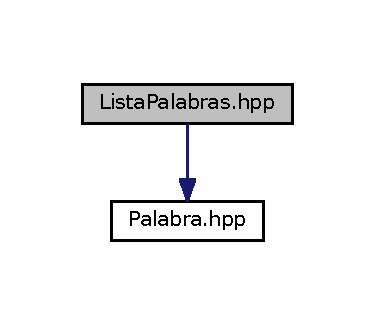
\includegraphics[width=180pt]{_lista_palabras_8hpp__incl}
\end{center}
\end{figure}
\subsection*{Clases}
\begin{DoxyCompactItemize}
\item 
class \hyperlink{class_lista_palabras}{Lista\-Palabras}
\begin{DoxyCompactList}\small\item\em Representa una colección de palabras distintas, cada una con un natural asociado. \end{DoxyCompactList}\end{DoxyCompactItemize}


\subsection{Descripción detallada}
Especificación de la clase \hyperlink{class_lista_palabras}{Lista\-Palabras}. 

Definición en el archivo \hyperlink{_lista_palabras_8hpp_source}{Lista\-Palabras.\-hpp}.


\hypertarget{_palabra_8hpp}{\section{Referencia del Archivo Palabra.\-hpp}
\label{_palabra_8hpp}\index{Palabra.\-hpp@{Palabra.\-hpp}}
}


Especificación de la clase \hyperlink{class_palabra}{Palabra}.  


\subsection*{Clases}
\begin{DoxyCompactItemize}
\item 
class \hyperlink{class_palabra}{Palabra}
\begin{DoxyCompactList}\small\item\em Representa una lista indexada de caracteres alfanuméricos. \end{DoxyCompactList}\end{DoxyCompactItemize}


\subsection{Descripción detallada}
Especificación de la clase \hyperlink{class_palabra}{Palabra}. 

Definición en el archivo \hyperlink{_palabra_8hpp_source}{Palabra.\-hpp}.


\hypertarget{pro2__s52_8cpp}{\section{Referencia del Archivo pro2\-\_\-s52.\-cpp}
\label{pro2__s52_8cpp}\index{pro2\-\_\-s52.\-cpp@{pro2\-\_\-s52.\-cpp}}
}


Programa principal para el ejercicio {\itshape Factor Psi}.  


Dependencia gráfica adjunta para pro2\-\_\-s52.\-cpp\-:\nopagebreak
\begin{figure}[H]
\begin{center}
\leavevmode
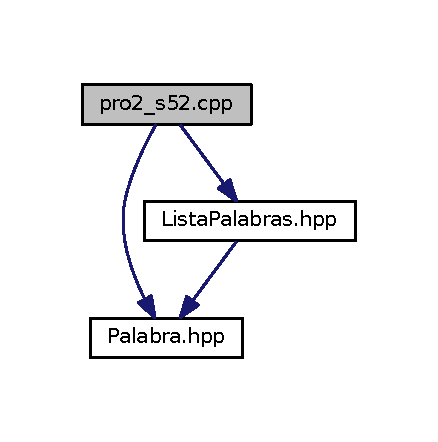
\includegraphics[width=210pt]{pro2__s52_8cpp__incl}
\end{center}
\end{figure}
\subsection*{Funciones}
\begin{DoxyCompactItemize}
\item 
int \hyperlink{pro2__s52_8cpp_ae66f6b31b5ad750f1fe042a706a4e3d4}{main} ()
\begin{DoxyCompactList}\small\item\em Programa principal para el ejercicio {\itshape Factor Psi}. \end{DoxyCompactList}\end{DoxyCompactItemize}


\subsection{Descripción detallada}
Programa principal para el ejercicio {\itshape Factor Psi}. 

Definición en el archivo \hyperlink{pro2__s52_8cpp_source}{pro2\-\_\-s52.\-cpp}.



\subsection{Documentación de las funciones}
\hypertarget{pro2__s52_8cpp_ae66f6b31b5ad750f1fe042a706a4e3d4}{\index{pro2\-\_\-s52.\-cpp@{pro2\-\_\-s52.\-cpp}!main@{main}}
\index{main@{main}!pro2_s52.cpp@{pro2\-\_\-s52.\-cpp}}
\subsubsection[{main}]{\setlength{\rightskip}{0pt plus 5cm}int main (
\begin{DoxyParamCaption}
{}
\end{DoxyParamCaption}
)}}\label{pro2__s52_8cpp_ae66f6b31b5ad750f1fe042a706a4e3d4}


Programa principal para el ejercicio {\itshape Factor Psi}. 



Definición en la línea 19 del archivo pro2\-\_\-s52.\-cpp.


\begin{DoxyCode}
\{

\}
\end{DoxyCode}

\addcontentsline{toc}{part}{Índice}
\printindex
\end{document}
